\documentclass[10pt]{article}

\usepackage{graphicx}
\usepackage{amsmath,amsfonts,amssymb}

% use different colors for links:
\usepackage{color}
\definecolor{darkgreen}{rgb}{0.1,0.5,0.1}
\definecolor{darkblue}{rgb}{0.2,0.2,1.0}
\usepackage[colorlinks=true,linkcolor=darkblue,citecolor=darkblue,
            filecolor=darkblue,urlcolor=darkgreen]{hyperref}


\setlength{\textwidth}{6.2in}
\setlength{\oddsidemargin}{0.3in}
\setlength{\evensidemargin}{0in}
\setlength{\textheight}{8.9in}
\setlength{\voffset}{-1in}
\setlength{\headsep}{26pt}
\setlength{\parindent}{0pt}
\setlength{\parskip}{5pt}



\input{../latex/macros.tex}  % input some useful macros

\begin{document}

% header:
\hfill\vbox{\hbox{AMath 586 / ATM 581}
\hbox{Homework \#5}\hbox{Due Tuesday, May 26, 2015}}

{\bf Name:} Your name here
\vskip 5pt

Homework is due to Canvas by 11:00pm PDT on the due date.

To submit, see \url{https://canvas.uw.edu/courses/962872/assignments/2869615}


%--------------------------------------------------------------------------
\vskip 1cm
\hrule
{\bf Problem 1}  

Let $U = [U_0,~U_1,~\ldots,~U_m]^T$ be a vector of function values at
equally spaced points on the interval $0\leq x \leq 1$, and suppose the
underlying function is periodic and smooth.  Then we can approximate 
the first derivative $u_x$ at all of these points by $DU$, where $D$ is
circulant matrix such as
\[
D_- = \frac 1 h \brm 1&&&&-1\\ -1&1\\ &-1&1\\ &&-1&1\\ &&&-1&1\erm,  \qquad
D_+ = \frac 1 h \brm -1&1\\ &-1&1\\ &&-1&1\\ &&&-1&1\\ 1&&&&-1\erm
\]
for first-order accurate one-sided approximations or
\[
D_0 = \frac 1 {2h} \brm 0&1&&&-1\\ -1&0&1\\ &-1&0&1\\ &&-1&0&1\\ 1&&&-1&0\erm
\]
for a second-order accurate centered approximation.  (These are illustrated
for a grid with $m+1=5$ unknowns and $h=1/5$.)


The advection equation $u_t + au_x=0$ on the interval $0\leq x \leq
1$ with periodic boundary conditions  
gives rise to the MOL discretization $U'(t) = -aDU(t)$
where $D$ is one of the matrices above.

\begin{enumerate} 
\item Discretizing $U' = -aD_-U$ by forward Euler gives the first order
upwind method
\[
U_j^{n+1} = U_j^n - \frac{ak}{h} (U_j^n - U_{j-1}^n),
\]
where the index $i$ runs from 0 to $m$ with addition of indices performed
mod $m+1$ to incorporate the periodic boundary conditions.

Suppose instead we discretize the MOL equation by the second-order Taylor
series method, 
\[
U^{n+1} = U^n - akD_-U^n + \half (ak)^2 D_-^2 U^n.
\]
Compute $D_-^2$ and also write out the formula for $U_j^n$ that results from
this method.  

\item How accurate is the method derived in part (a) compared to the
Beam-Warming method, which is also a 3-point one-sided method?

\item Suppose we make the method more symmetric:
\[
U^{n+1} = U^n - \frac{ak}{2} (D_+ +D_-)U^n + \half (ak)^2 D_+D_- U^n.
\]
Write out the formula for $U_j^n$ that results from this method.  
What standard method is this?

\end{enumerate}



% uncomment the next two lines if you want to insert solution...
%\vskip 1cm
%{\bf Solution:}

% insert your solution here!

%--------------------------------------------------------------------------
\vskip 1cm
\hrule
{\bf Problem 2}  


\begin{enumerate} 
\item
Produce a plot similar to those shown in Figure 10.1 for the upwind method
(10.21) with the same values of $a=1$, $h=1/50$ and $k=0.8h$
used in that figure.

\item Produce the corresponding plot if the one-sided method (10.22) is
instead used with the same values of $a,~h$, and $k$.
\end{enumerate}

% uncomment the next two lines if you want to insert solution...
%\vskip 1cm
%{\bf Solution:}

% insert your solution here!
%--------------------------------------------------------------------------
\vskip 1cm
\hrule
{\bf Problem 3}  

Suppose $a>0$ and consider the following {\it skewed leapfrog} method for
solving the advection equation $u_t + au_x = 0$:
\[
U_j^{n+1} = U_{j-2}^{n-1}  - \left(\frac{ak}{h} - 1\right) (U_j^n -
U_{j-2}^n).
\]
The stencil of this method is
\vskip 5pt
\hfil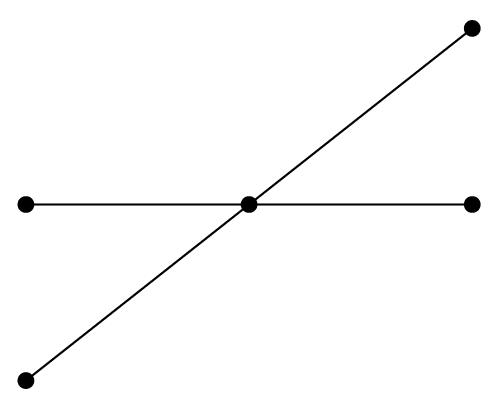
\includegraphics[width=1.5in]{skewedlfstencil.png}\hfil
\vskip 5pt

Note that if $ak/h \approx 1$ then this stencil roughly follows the
characteristic of the advection equation and might be expected to be more
accurate than standard leapfrog.  (If $ak/h = 1$ the method is exact.)


\begin{enumerate}

\item What is the order of accuracy of this method?

\item For what range of Courant number $ak/h$ does this method satisfy the
CFL condition?

\item Show that the method is in fact stable for this range of Courant
numbers by doing von Neumann analysis.  
{\bf Hint:} Let $\gamma(\xi) = e^{i\xi h}g(\xi)$ and show that $\gamma$
satisfies a quadratic equation closely related to the equation (10.34)
that arises from a von Neumann analysis of the leapfrog method.

\end{enumerate}

% uncomment the next two lines if you want to insert solution...
%\vskip 1cm
%{\bf Solution:}

% insert your solution here!
%--------------------------------------------------------------------------
\vskip 1cm
\hrule
{\bf Problem 4}  


Derive the modified equation (10.45) for the Lax-Wendroff method.


% uncomment the next two lines if you want to insert solution...
%\vskip 1cm
%{\bf Solution:}

% insert your solution here!
%--------------------------------------------------------------------------
\vskip 1cm
\hrule
{\bf Problem 5}  


The m-file \verb+advection_LW_pbc.m+ from the book repository
implements the Lax-Wendroff method for
the advection equation on $0\leq x\leq 1$ with 
periodic boundary conditions.

The class repository contains a Python translation, \verb+$AM586/codes/advection_LW_pbc.py+.

You might want to first experiment with these and see how Lax-Wendroff behaves for various grid resolutions.  Note that the way this problem is set up, the solution advects twice around the domain over time 1 and should end up agreeing with the initial data. 

\begin{enumerate}
\item Modify one of these files to 
implement the leapfrog method and verify that this is second order accurate.
Note that you will have to specify two levels of initial data.  For the
convergence test set $U^1_j = u(x_j,k)$, the true solution at time $k$.

\item Modify your code so that the initial data consists of
a wave packet
\[
\eta(x) = \exp(-\beta(x-0.5)^2) \sin(\xi x)
\]
Work out the true solution $u(x,t)$ for this data.
Using $\beta = 100$, $\xi=80$ and $U^1_j = u(x_j,k)$, test that your code
still exhibits second order accuracy for $k$ and $h$ sufficiently small.

\item Using $\beta = 100$, $\xi=150$ and $U^1_j = u(x_j,k)$, estimate the
group velocity of the wave packet computed with leapfrog using $m=199$ and
$k = 0.4h$.  How well does this compare with the  value (10.52) predicted by
the modified equation?  

{\bf Note:} Early editions of the text book had a typo in (10.52).  There should be a factor $\nu^2$ in the denominator.

\end{enumerate} 

% uncomment the next two lines if you want to insert solution...
%\vskip 1cm
%{\bf Solution:}

% insert your solution here!

%--------------------------------------------------------------------------

\end{document}

